\chapter{结果分析}
\label{cha:fourthsection}

\section{训练样本数量的影响}


\section{网络结构影响}

\section{激活函数影响}
实验得到的不同激活函数下的MSE与MAE如下：


\section{欠拟合与过拟合分析}

\section{训练时间比较}
此外，实验记录了在不同网络结构或激活函数下的模型训练时间，不同网络结构下模型训练时间如下图所示
由图可说明，当网络的宽度或深度增加时，模型训练时间也会增加，而网络深度对训练时间的影响比宽度的影响大




如图\ref{Fig4-1}所示：
\begin{figure}[!htbp]
    \centering
    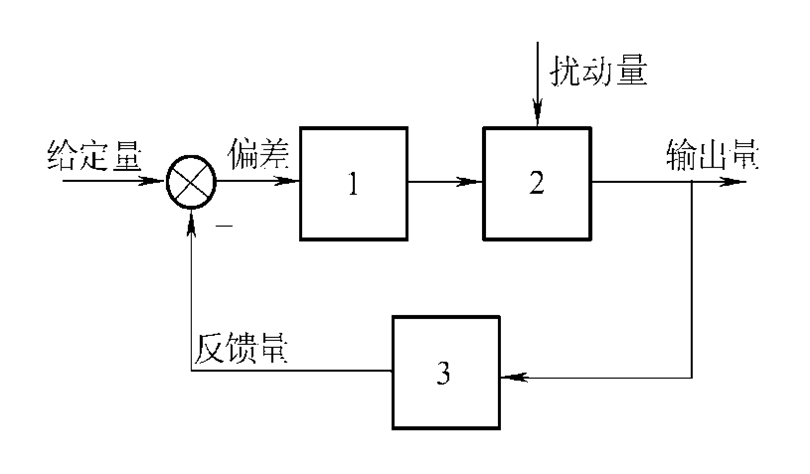
\includegraphics{figures/Fig4-1.png}
    \caption{闭环系统示意图}\label{Fig4-1}
\end{figure}
制作图时请注意:





\section{关于表格}
\label{sec:results}
如表\ref{Tab4-1}所示：
\begin{table}[htbp]
  \centering
  \caption{表格示例}
    \begin{tabular}{ccccc}
    \toprule
    Aaa & Bbb & Ccc & Ddd & Eee \\
    \midrule
    1-1  & 1-2  & 1-3 & 1-4 & 1-5 \\
    2-1  & 2-2  & 2-3 & 2-4 & 2-5 \\
    3-1  & 3-2  & 3-3 & 3-4 & 3-5 \\
    4-1  & 4-2  & 4-3 & 4-4 & 4-5 \\
    \bottomrule
    \end{tabular}%
  \label{Tab4-1}%
\end{table}%





参考文献（举例）
\begin{enumerate}
\renewcommand{\labelenumi}{[\theenumi]}
\item	闫明礼, 张东刚. CFG桩复合地基技术及工程实践（第二版）. 北京: 中国水利水电出版社, 2006
\end{enumerate}